% !TeX root = ../thuthesis-example.tex

\chapter{遗忘方法的实现与验证}

\section{实验验证}

\subsection{实验环境介绍}
我们用到的实验设备是两台服务器,
\\cpu Intel(R) 
\\Core(TM) i9-9900K CPU @ 3.60GHz
\\Intel(R) Core(TM) i7-6700K CPU @ 4.00GHz
\\内存 32g 32g
\\硬盘 ssd ssd
\\显卡  1xNvidia Geforce 2080 3xNvidia Geforce 1080
\\操作系统 ubuntu16.04LTS ubuntu16.04LTS
\\深度学习框架pytorch
\\数据集是cifar-10,正常训练集50000张图片,测试集10000张图片。遗忘两个类别,遗忘集是从正常训练集分离出来的10000张图片,遗忘测试集2000张图片。保留训练集是指正常训练集出去了遗忘集外的数据集合。保留训练集40000张图片,保留测试集8000张图片。神经网络有Resnet18和Resnet50。
\subsection{实验设计}

\subsubsection{确定冻结层数实验}
实验一:确定冻结层数实验
\\实验目的:这个实验的目的是确定网络冻结的层次数。确定的标准是根据3.5中讲到的四个指标的综合指标。
\\实验准备:正常训练集,遗忘集和保留集,还有测试集。使用的神经网络框架是Resnet18。
\\实验过程:首先使用正常训练集去训练神经网络,直至训练集准确率收敛,获得模型1,在训练网络之前保存神经网络训练之前的网络参数,记为模型0。再使用保留集重新训练一个神经网络,获得模型2。将模型1的最后一层(全联接层)的参数替换为模型0的最后一层参数,模型1其余层数的参数不变,由此得到模型1\_reset\_fc\_before\_training。将模型1\_reset\_fc\_before\_training加载到一个新的神经网络中,使用保留集去训练这个新的网络,直至训练准确率收敛,在训练过程中保持除全连接层以外层次的参数不被更新(即冻结),得到模型1\_reset\_fc\_after\_training。将模型1\_reset\_fc\_after\_training加载到模型,分别测量并记录指标一、指标二、指标三和指标四。
\\实验结束:计算并记录综合指标计算结果。
\subsubsection{冻结必要性验证实验}
实验目的:通过本实验验证冻结较低层次的参数是否对加快遗忘训练收敛速度有一定的贡献,同时观察遗忘集集准确率、保留集准确率和测试集准确率的变化情况。
\\实验准备:数据集有正常训练集,保留集。神经网络是Resnet18。
\\实验过程:
\\1. 用正常训练集训练神经网络得到模型1
\\2. 在正常训练集训练之前保留网络参数得到模型0
\\3. 用模型0的全连接层参数,替换模型1的全连接层的参数,得到模型1\_reset\_fc\_before\_training
\\4. 用神经网络加载模型1\_reset\_fc\_before\_training,网络参数全部无需冻结,用保留集训练至训练准确率收敛,得到模型1\_reset\_fc\_after\_training
\\5. 分别记录下各个指标
\\6. 分别将神经网络从最后一层到各个层的参数重置后,重复上述3-5步骤,将全连接层替换成全连接层至各个层之间的参数
\\实验结束:计算并记录各个模型综合指标计算结果
\subsubsection{反向冻结验证实验}
实验目的:验证卷积神经网络的分层抽象特性,与正向冻结实验进行对照。
\\实验准备:数据集有正常训练集,保留集。神经网络是Resnet18。
\\实验过程:
\\1. 用正常训练集训练神经网络得到模型1
\\2. 在正常训练集训练之前保留网络参数得到模型0
\\3. 用模型0的第一卷积层参数,替换模型1的第一卷积层参数,得到模型1\_reset\_conv1\_before\_reverse\_training
\\4. 用神经网络加载模型1\_reset\_conv1\_before\_reverse\_training,除了第一卷积层外,其余层数的参数全部冻结。用保留集训练至训练准确率收敛,得到模型1\_reset\_conv1\_after\_reverse\_training
\\5. 分别记录下各个指标
\\6. 分别重置第一卷积层至最后一层全连接层参数,重复上述第3-5步骤。
\\实验结束:计算并记录各个模型综合指标计算结果
\subsubsection{遗忘可持续性验证实验}
实验目的:检验冻结重置方法随着遗忘类别数量的增多有效性的变化情况
\\实验准备:数据集有正常训练集,分别遗忘掉1-9个类别的保留集1-保留集9共9个保留集。神经网络是Resnet18。
\\实验过程:
\\1. 用正常训练集训练神经网络得到模型1
\\2. 在正常训练集训练之前保留网络参数得到模型0
\\3. 使用保留集1-保留集9分别重新训练模型,得到模型\_forget\_1\_retrain,...,模型\_forget\_9\_retrain。
\\4. 用神经网络加载模型1,然后把神经网络全连接层和6层卷积层的参数重置为模型0的相应层次的参数。
\\5. 分别用保留集1-保留集9去训练步骤4中生成的网络,训练过程中冻结除了全连接层和后6层卷积层的参数。得到模型1\_fc\_conv6\_retain\_1\_finetune,...,模型1\_fc\_conv6\_retain\_9\_finetune共9个神经网络的参数。
\\6. 5中得到的网络参数进行指标测试,并记录。
\\实验结束:计算并记录各个模型综合指标的计算结果
\section{实验结果}
\subsection{确定冻结层数实验}
\begin{figure}
    \centering
    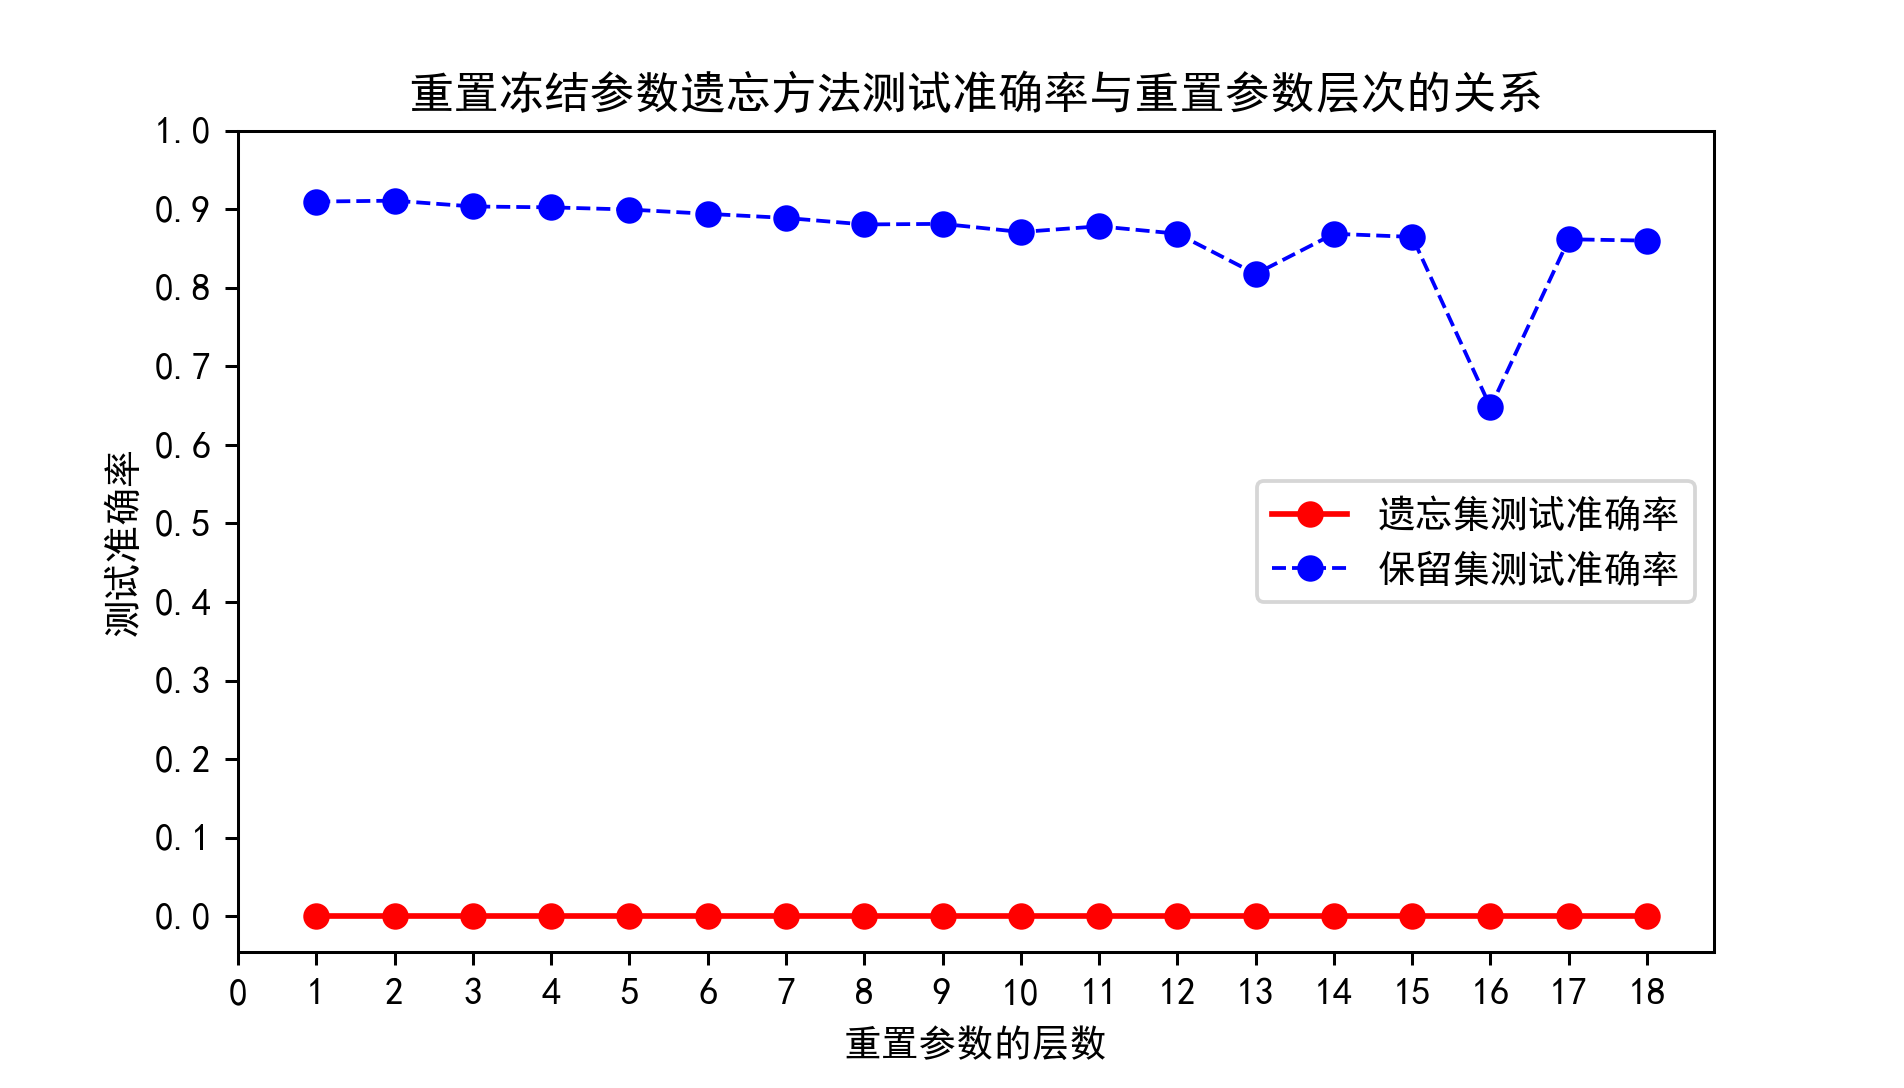
\includegraphics[width=0.9\linewidth]{chapter4_1.png}
    \caption{重置冻结参数遗忘方法测试准确率与重置参数层次的关系}
    \label{fig:chapter4_1}
\end{figure}
如图\ref{fig:chapter4_1}所示,图中展示了本文所讲述的重置冻结参数遗忘方法训练的网络用遗忘集和保留集训练之后得到测试准确率。
蓝色的折线代表利用保留测试集测试的准确率,红色的折线代表使用遗忘测试集测试的准确率的情况。
从红线可以看出,遗忘测试集的准确率全是0。这样的结果与完全重新训练得到的模型在遗忘测试集上的准确率完全相同。这说明使用本文提出的冻结重置参数方法,无论重置多少层参数,在遗忘集上均能达到理想的效果。
从蓝线与上面的点线可以看出,本方法得到的模型在保留集测试准确率上在大部分情况下均好于完全重新训练得到的模型在保留集上的准确率。
从蓝色圆点曲线中也发现随着重置参数的层数的增加,其保留集测试准确率有下降趋势,逐渐接近完全重新训练模型在保留集上的测试结果。
仅通过这一个方面还不足以让我们选出要重置参数的层次。
\begin{figure}
    \centering
    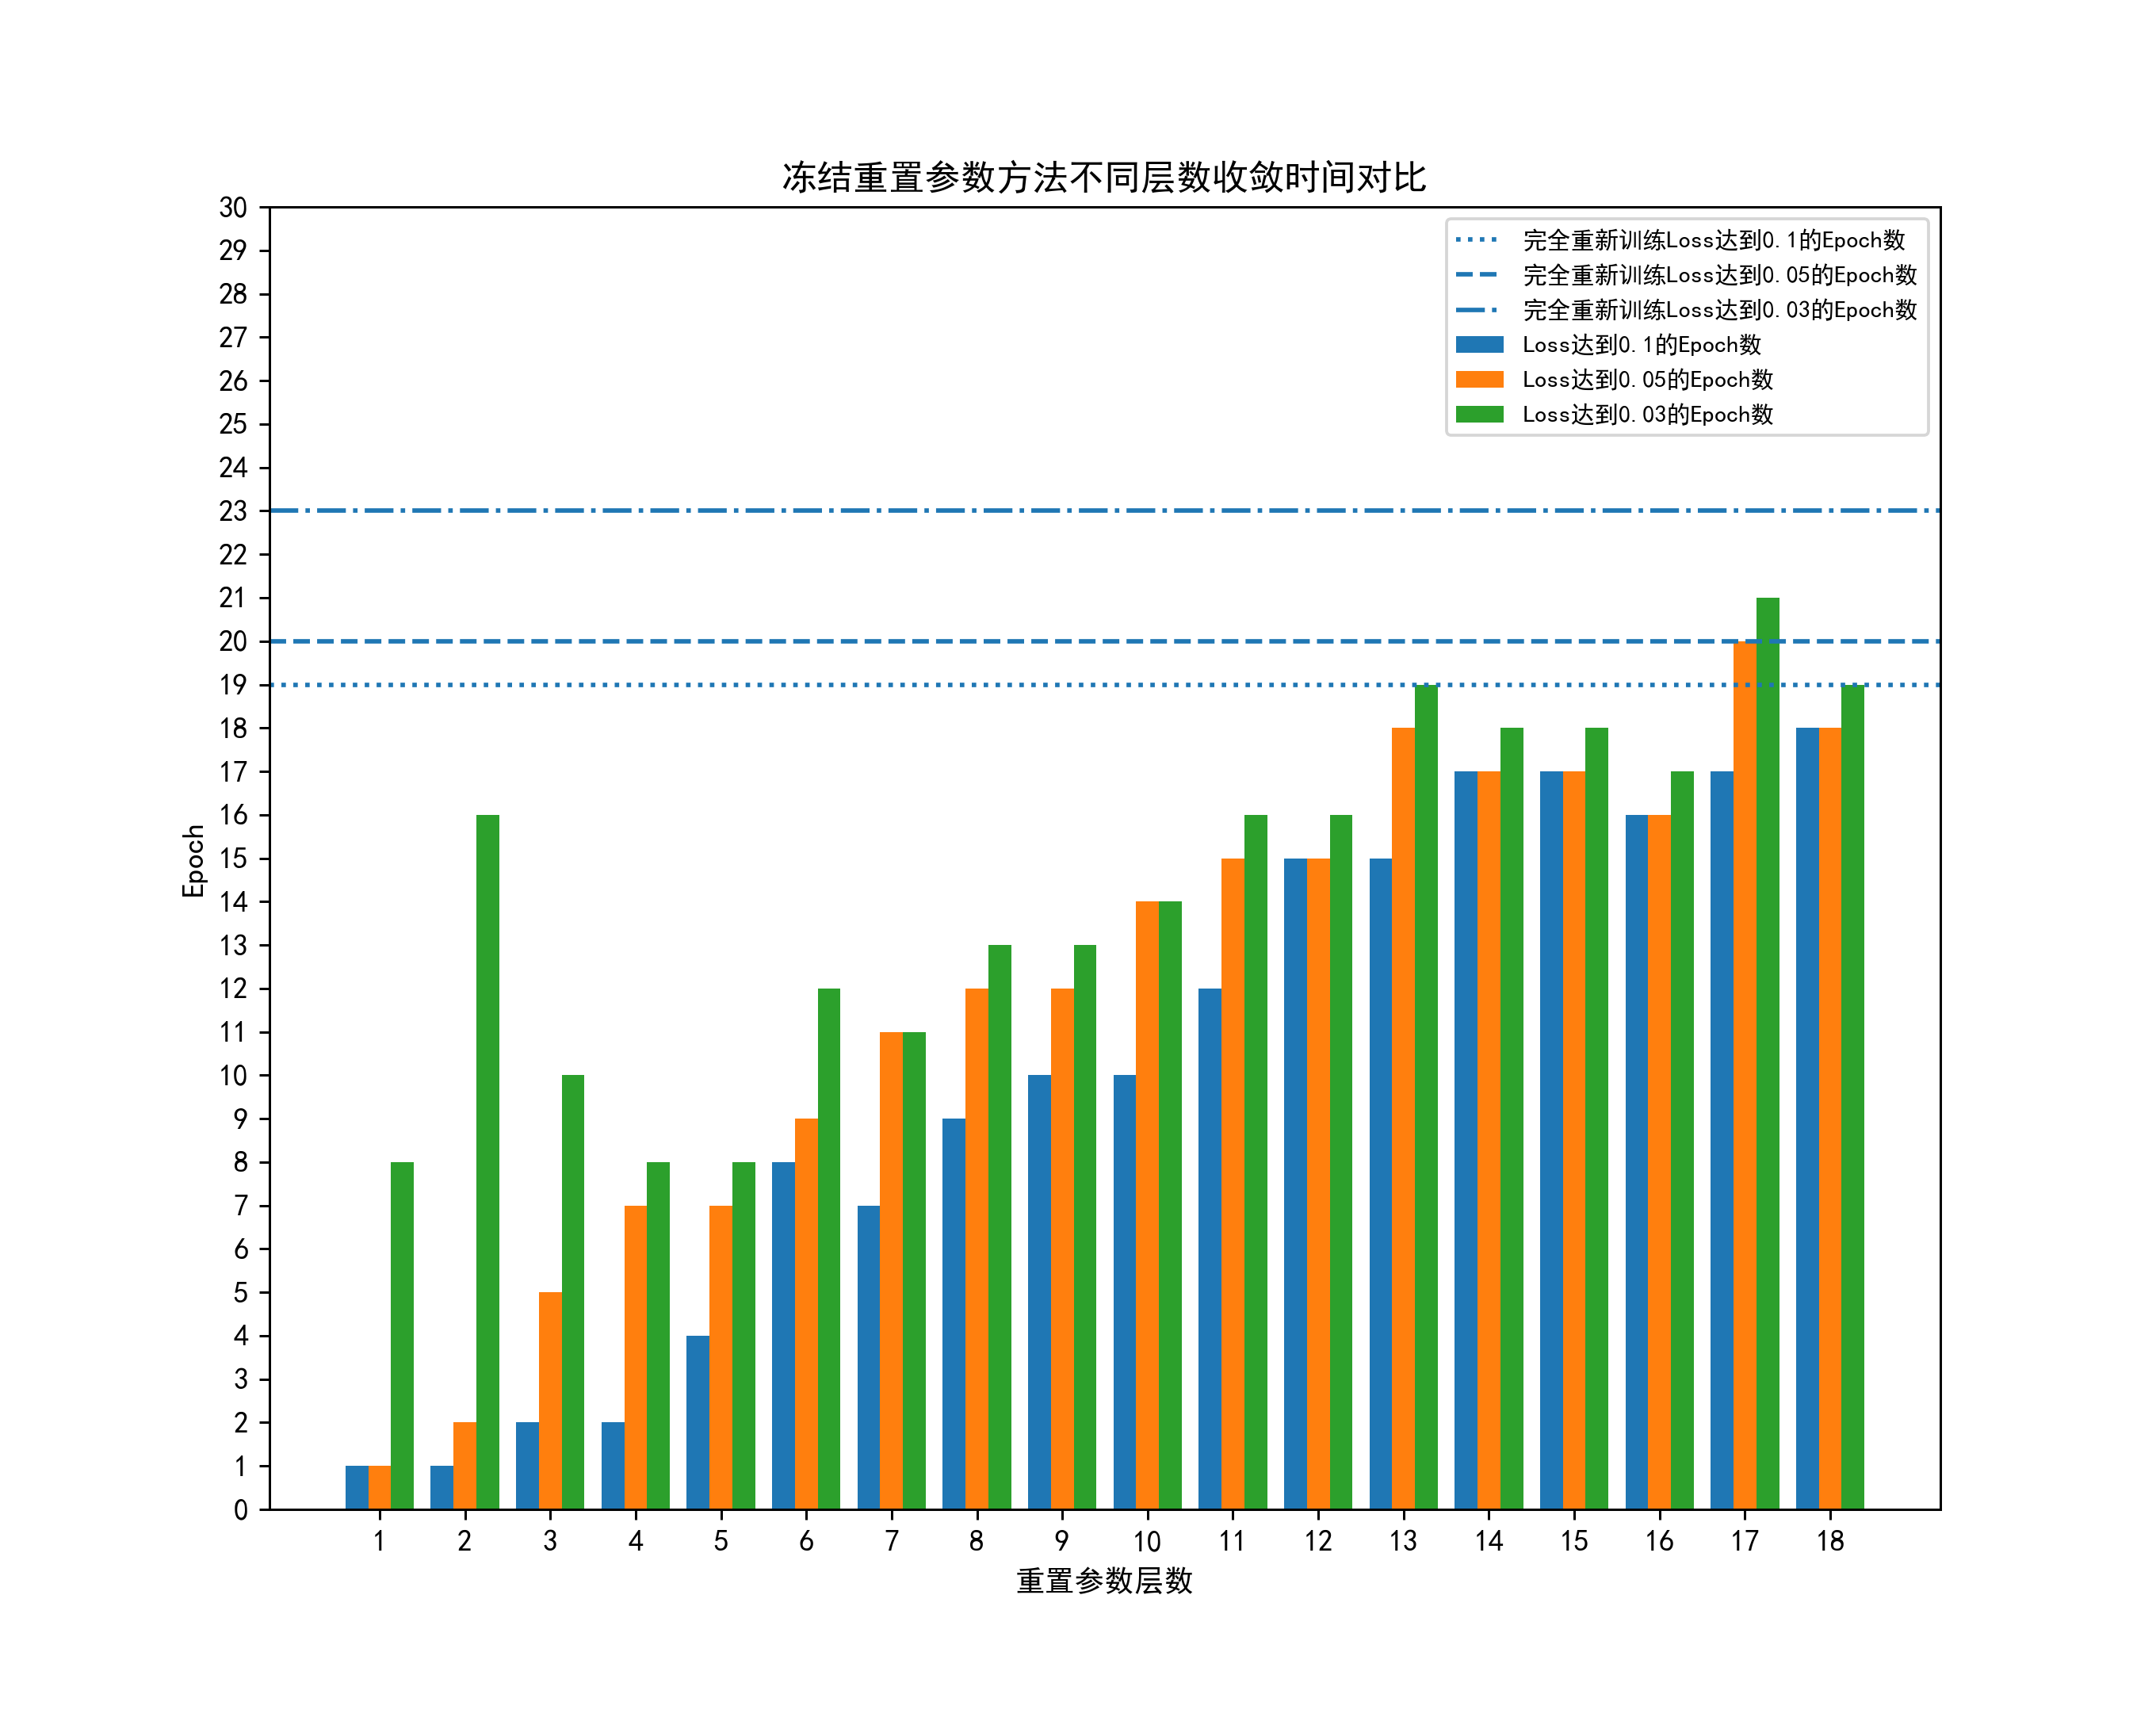
\includegraphics[width=1\linewidth]{chapter4_time_1.png}
    \caption{冻结重置参数方法不同层数收敛时间对比}
    \label{fig:chapter4_time_1}
\end{figure}
\\    如图\ref{fig:chapter4_time_1}所示,图中展示了本文所讲述的重置冻结参数遗忘方法在重置不同层次参数上使用保留集训练后收敛时间的对比。
图中展示了三套柱状对比图,蓝色柱图、黄色柱图和绿色柱图分别代表使用保留训练集训练网络时,该训练批次(Epoch)的平均损失函数loss的值首次降到0.1,0.05和0.03以下时的训练批次(Epoch)数。
批次数越小,说明训练的收敛时间越快。上面有三条不同线型的横线,分别代表为了遗忘一定的类别完全重新训练网络,该训练过程的平均损失函数值首次降到0.1,0.05和0.03以下时的训练批次(Epoch)数。
这三条横线的作用时与本文提到的方法进行收敛时间上的对比。
从图中的柱状图中可以看出,随着重置参数的层数逐渐增多,其收敛的Epoch逐渐增大,逐渐接近完全重新训练时收敛的Epoch。
其实这也不难理解,随着重置参数的层数增多,网络中需要更新的参数也逐渐增多,其状态也越来越接近完全重新训练的情况,所以收敛时间也逐步接近完全重新训练。
我们希望选择的层次是选择该层次后,训练后的准确率越高越好,训练收敛时间越快越好。
所以综合图\ref{fig:chapter4_1}和\ref{fig:chapter4_distance_1},可以备选的层次是前7层均在可以接受的范围内,重置参数层数越小,准确率越高,收敛时间也越快。
\begin{figure}
    \centering
    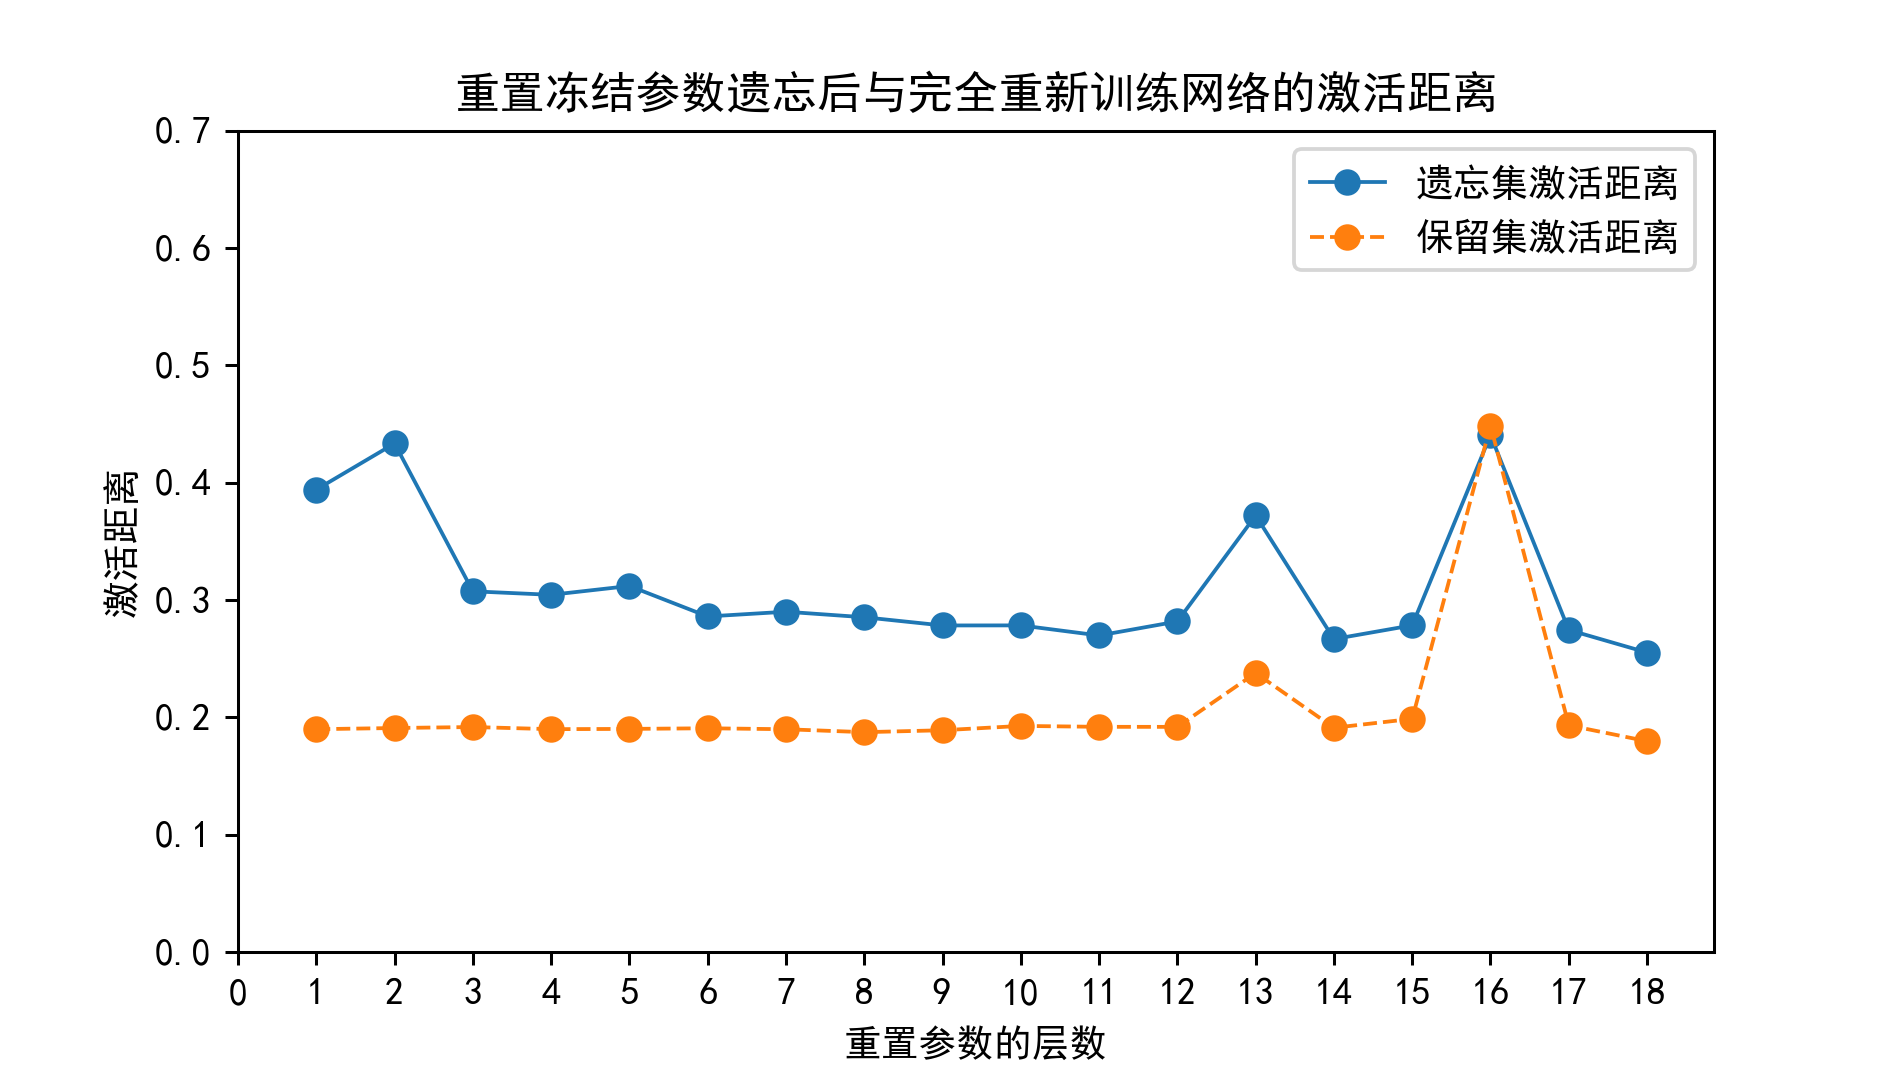
\includegraphics[width=0.9\linewidth]{chapter4_distance_1.png}
    \caption{重置冻结参数遗忘后与完全重新训练网络的激活距离}
    \label{fig:chapter4_distance_1}
\end{figure}
\\    如图\ref{fig:chapter4_time_1}所示,图中展示了本文所讲述的重置冻结参数遗忘方法训练的网络与完全重新训练所训练的网络之间对于测试集输出之间的距离差。
这个距离差在上一节有具体讲到,是两个网络输出向量差的绝对值的第二范数值。我们用这个范数值在测试数据集上的期望来作为两个网络的激活距离。
蓝色折线代表两个网络在遗忘集上的激活距离,橙色折线代表两个网络在保留集上的激活距离。从图中可以看出,两个网络在遗忘集上的激活距离要高于在保留集上的激活距离。
我们对于两个网络激活距离的期望是越小越好,在前7层可以看到保留集的激活距离普遍稳定地保持较低数值,而对于遗忘集的激活距离前2层的数值相对较大,3、4、5层数值也略大,从第6层开始,数值变得平稳。
因此,综合图\ref{fig:chapter4_1}和图\ref{fig:chapter4_time_1}和图\ref{fig:chapter4_distance_1}的分析结果,我们选择第6层作为重置冻结参数遗忘方法对于ResNet18网络重置参数的层数。
\subsection{冻结必要性验证实验}
\begin{figure}
    \centering
    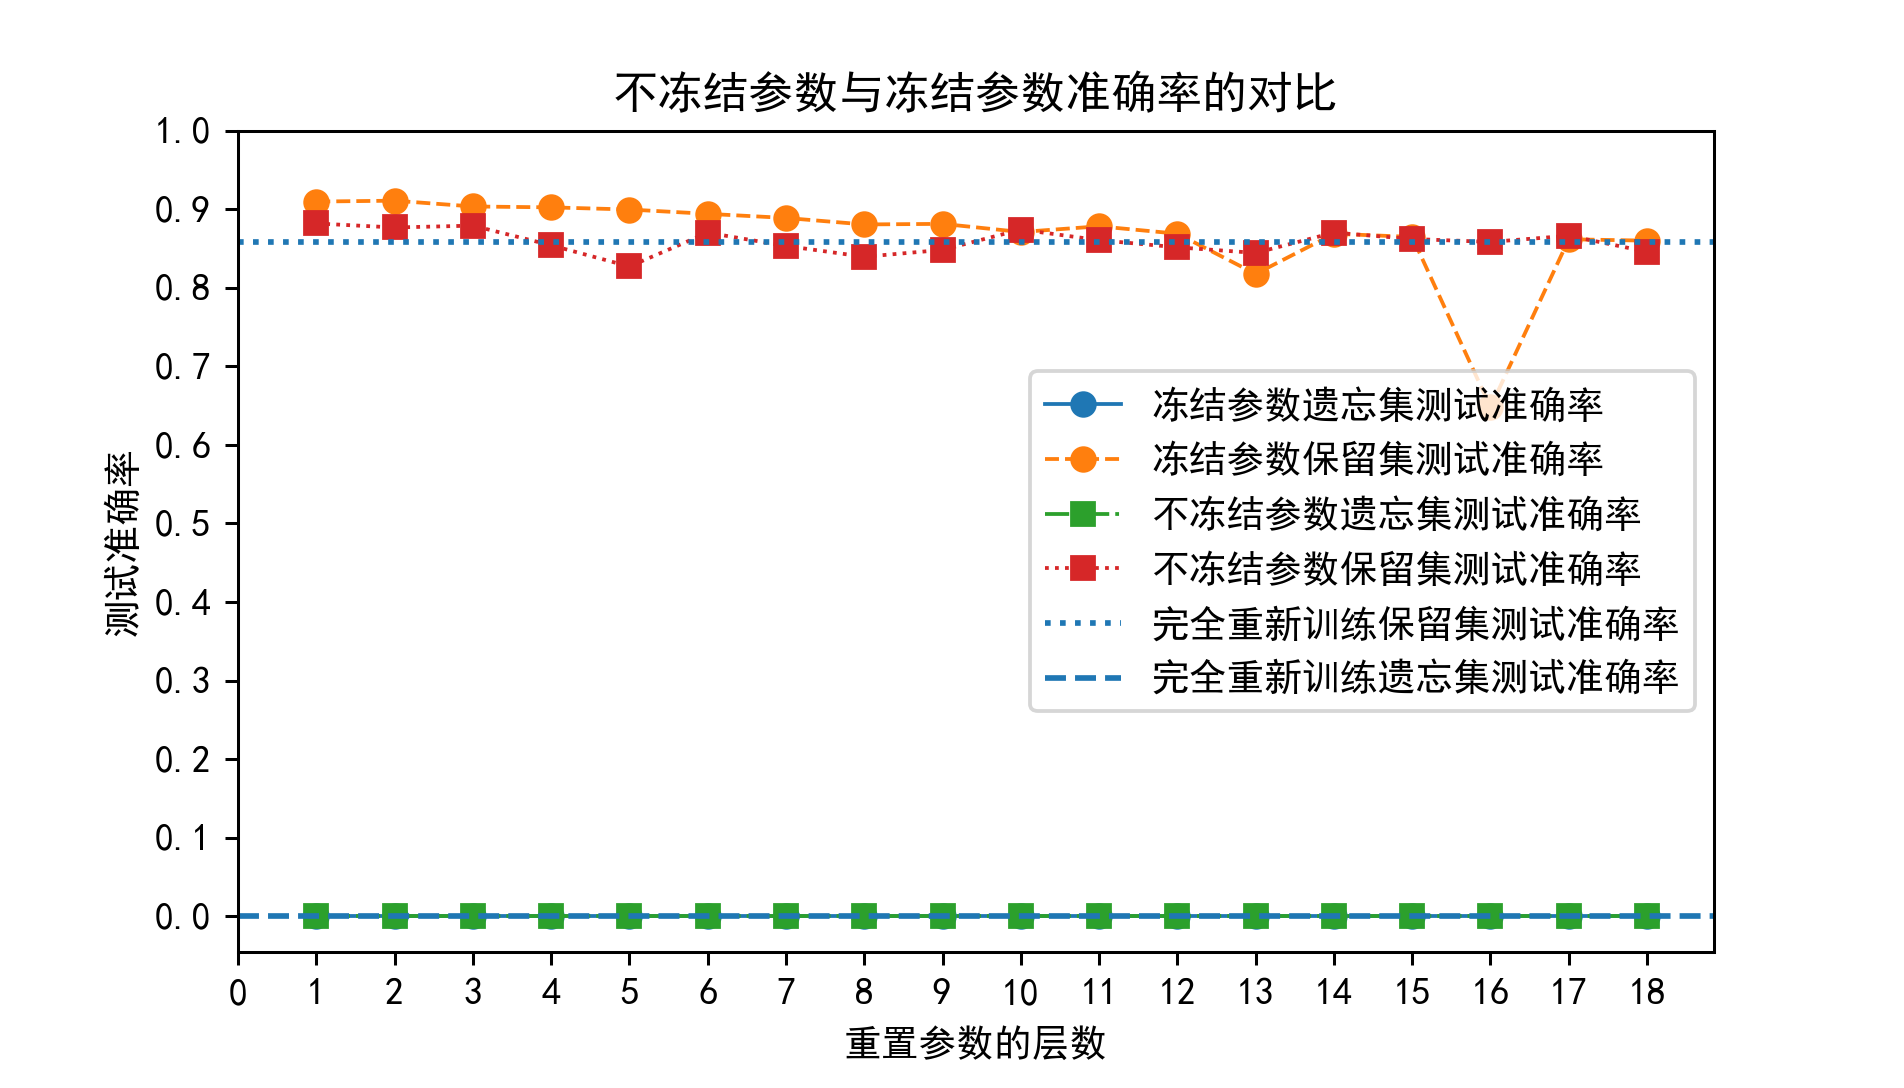
\includegraphics[width=0.9\linewidth]{chapter4_2.png}
    \caption{不冻结参数与冻结参数准确率的对比}
    \label{fig:chapter4_2}
\end{figure}
如图\ref{fig:chapter4_2}所示,图中展示了重置一定参数后冻结参数与不冻结参数训练对遗忘类别和保留类别准确率的影响。
橘黄色圆点折线代表冻结参数后使用保留训练集训练网络得到的网络在保留测试集上得到的准确率,蓝色圆点折线代表该网络的在遗忘测试集上得到的测试准确率。
红色方格折线代表不冻结参数的情况下使用保留训练集训练得到的网络在保留测试集上得到的测试准确率,绿色方格折线代表该网络在遗忘测试集上得到的测试准确率。
除此之外,图中还画了两条横线,圆点线代表完全重新训练的网络模型在保留测试集上得到的测试准确率,条状线段线代表完全重新训练的网络模型在遗忘测试集上得到的测试准确率。
这两条横线的主要作用是作为冻结参数和不冻结参数准确率的参照。通过橘黄色圆点折线和红色方格折线可以看出冻结参数与不冻结参数在保留集测试准确率上总体相差不大,但是冻结参数的方法要略好于不冻结参数方法。
在遗忘集的测试准确率上,两种方法效果相同,均为0。
\begin{figure}
    \centering
    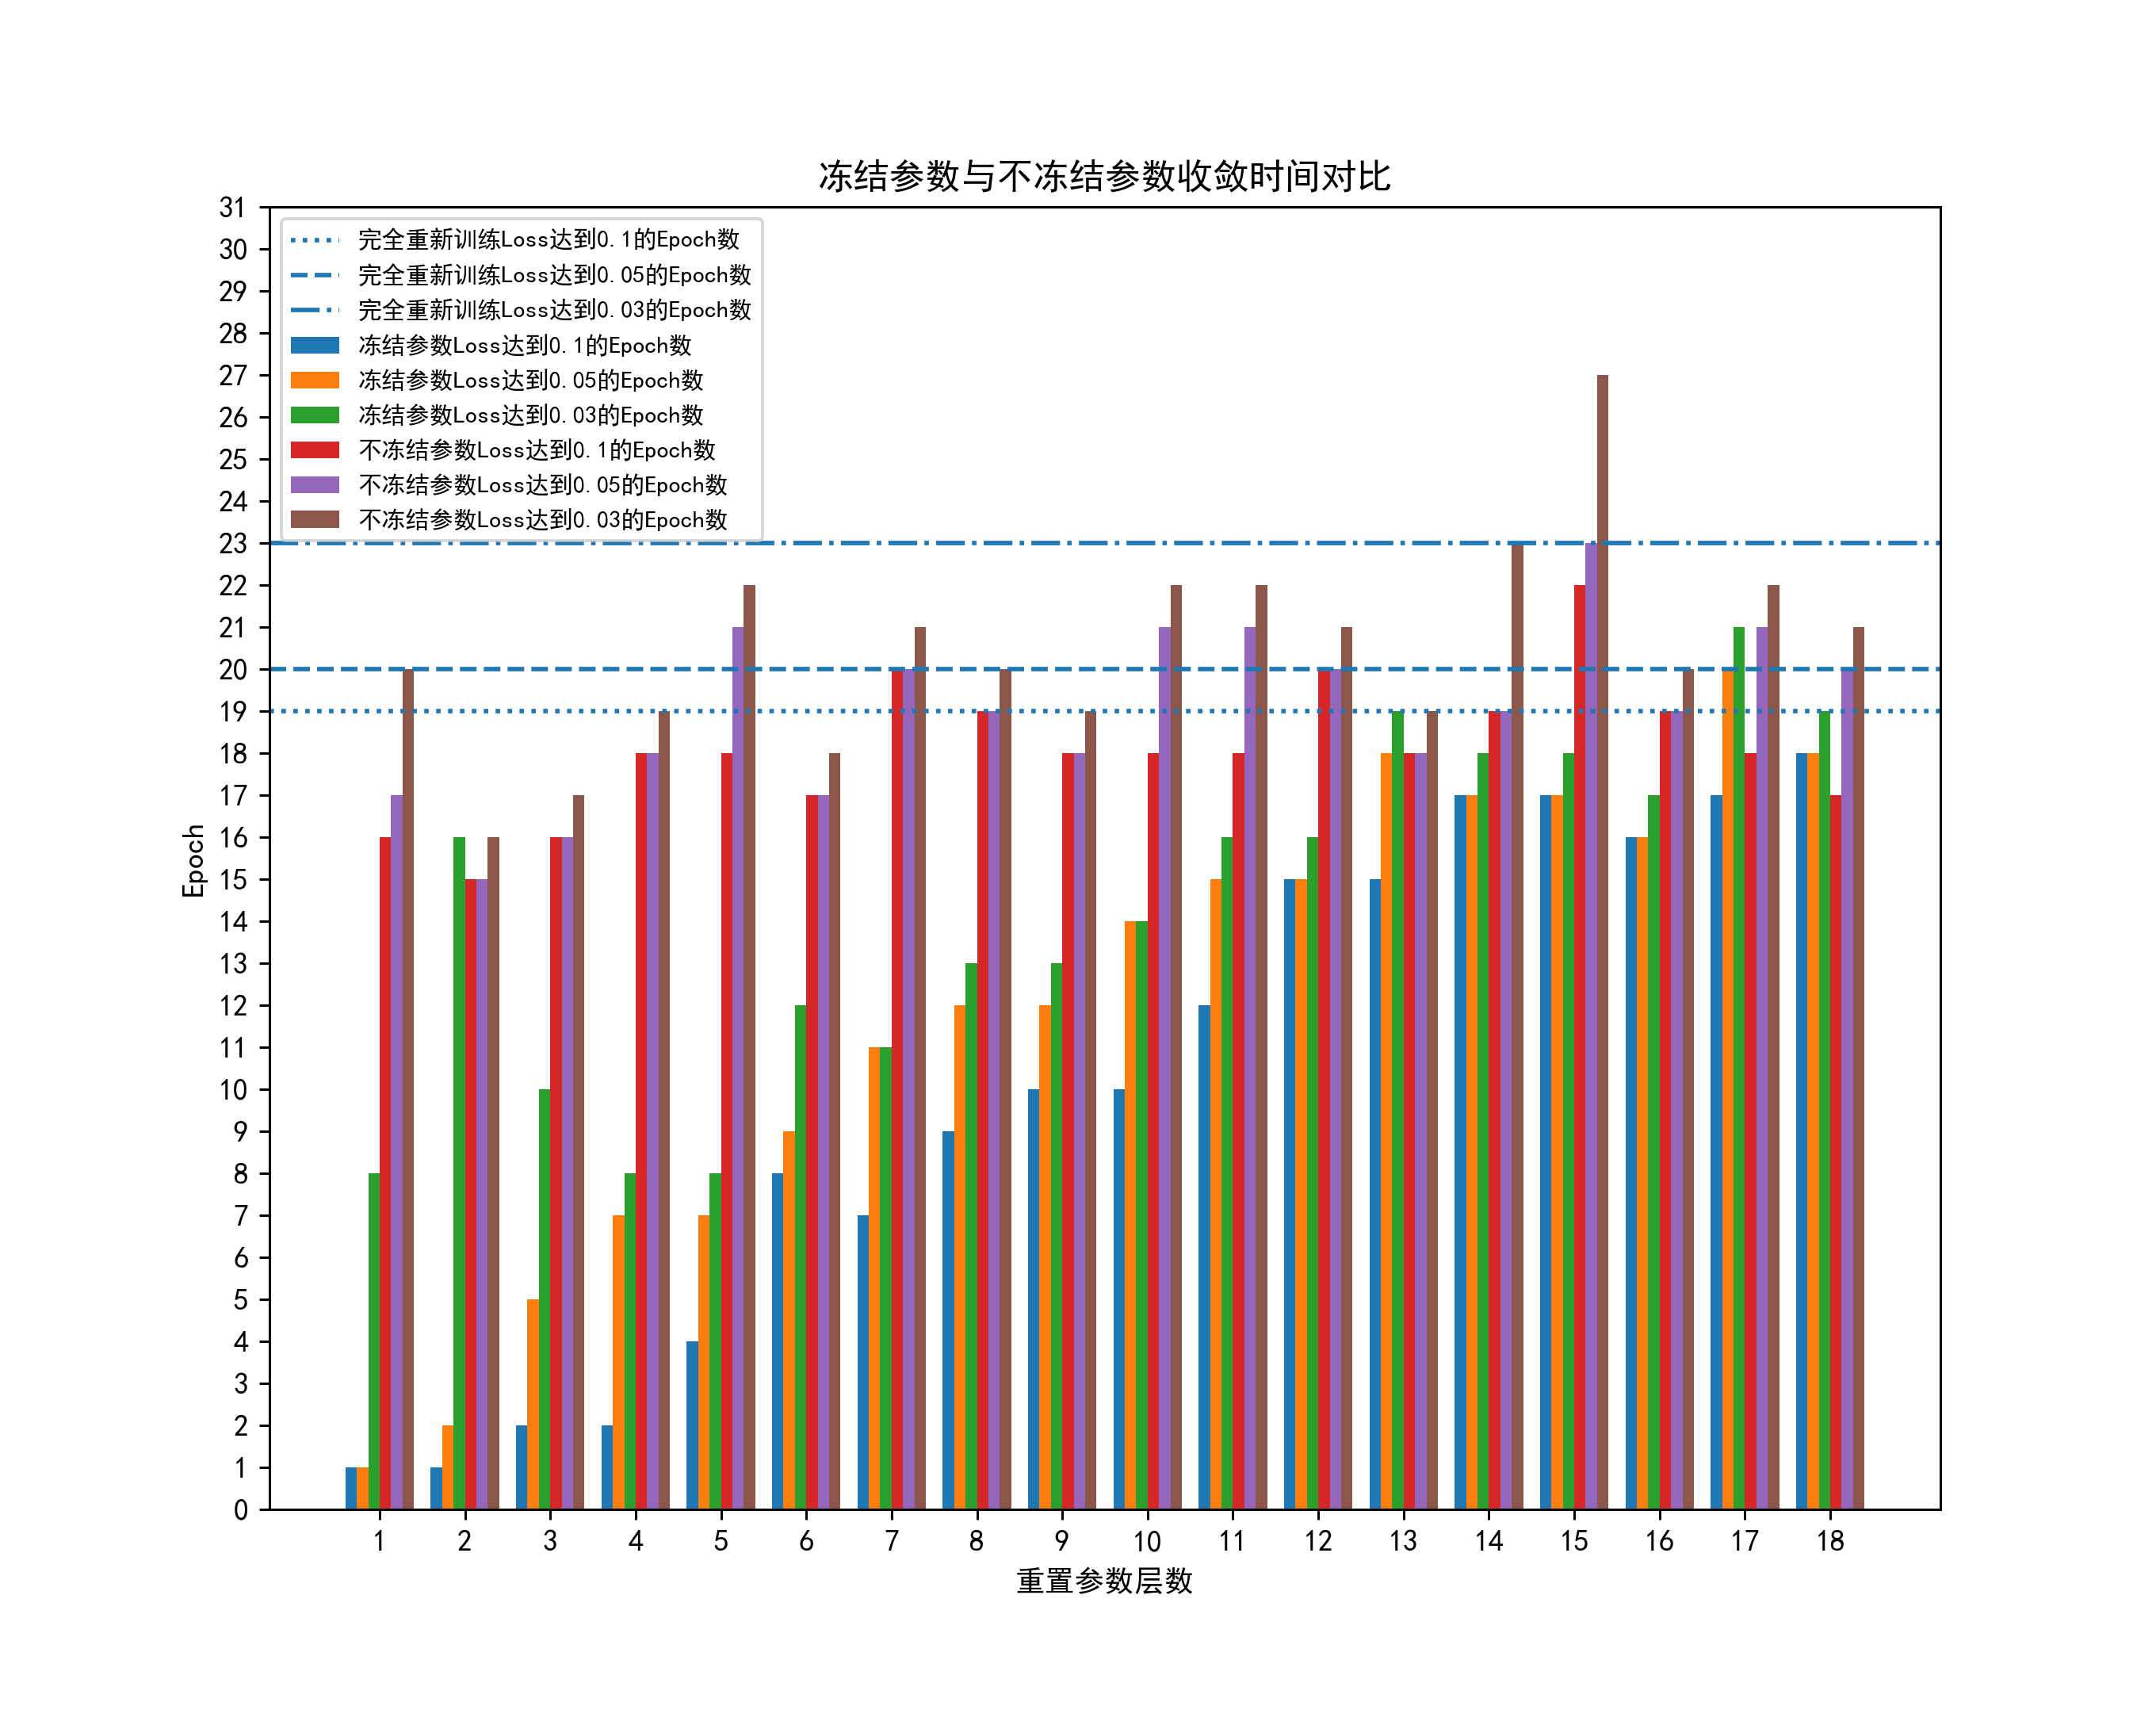
\includegraphics[width=1\linewidth]{chapter4_time_2.png}
    \caption{冻结参数与不冻结参数收敛时间对比}
    \label{fig:chapter4_time_2}
\end{figure}
\\如图\ref{fig:chapter4_time_2}所示,图中展示了冻结参数与不冻结参数重置参数后使用保留训练集训练网络的收敛时间。这个收敛时间同实验一的收敛时间定义相同。
蓝色、黄色和绿色柱图分别代表冻结参数情况下网络的平均损失函数值收敛到0.1、0.05和0.03时所花费的训练周期,即Epoch数。
粉色、紫色和棕色柱图分别代表非冻结参数情况下网络的平均损失函数收敛到0.1、0.05和0.03时所花费的训练周期数。
上面画出的三条横线,圆点线、条状线和点段线分别代表完全重新训练网络过程中,网络的平均损失函数值收敛至0.1、0.05和0.03时所花费的训练周期数。其主要作用是用来提供参照。
通过观察冻结参数和不冻结参数的柱状图可以发现,冻结参数后训练的收敛时间从整体上要少于不冻结参数训练网络收敛时间。这个现象也是符合分析的逻辑,冻结参数后,一部分参数不需要计算更新,而没有冻结参数的网络则需要计算所有参数的更新,从计算量上分析,不冻结参数训练网络所需要的工作量是比冻结参数要大的。
通过图\ref{fig:chapter4_2}和图\ref{fig:chapter4_time_2}的分析结果可以初步得出结论,冻结参数训练网络的方法要好于不冻结参数训练网络的方法。
\begin{figure}
    \centering
    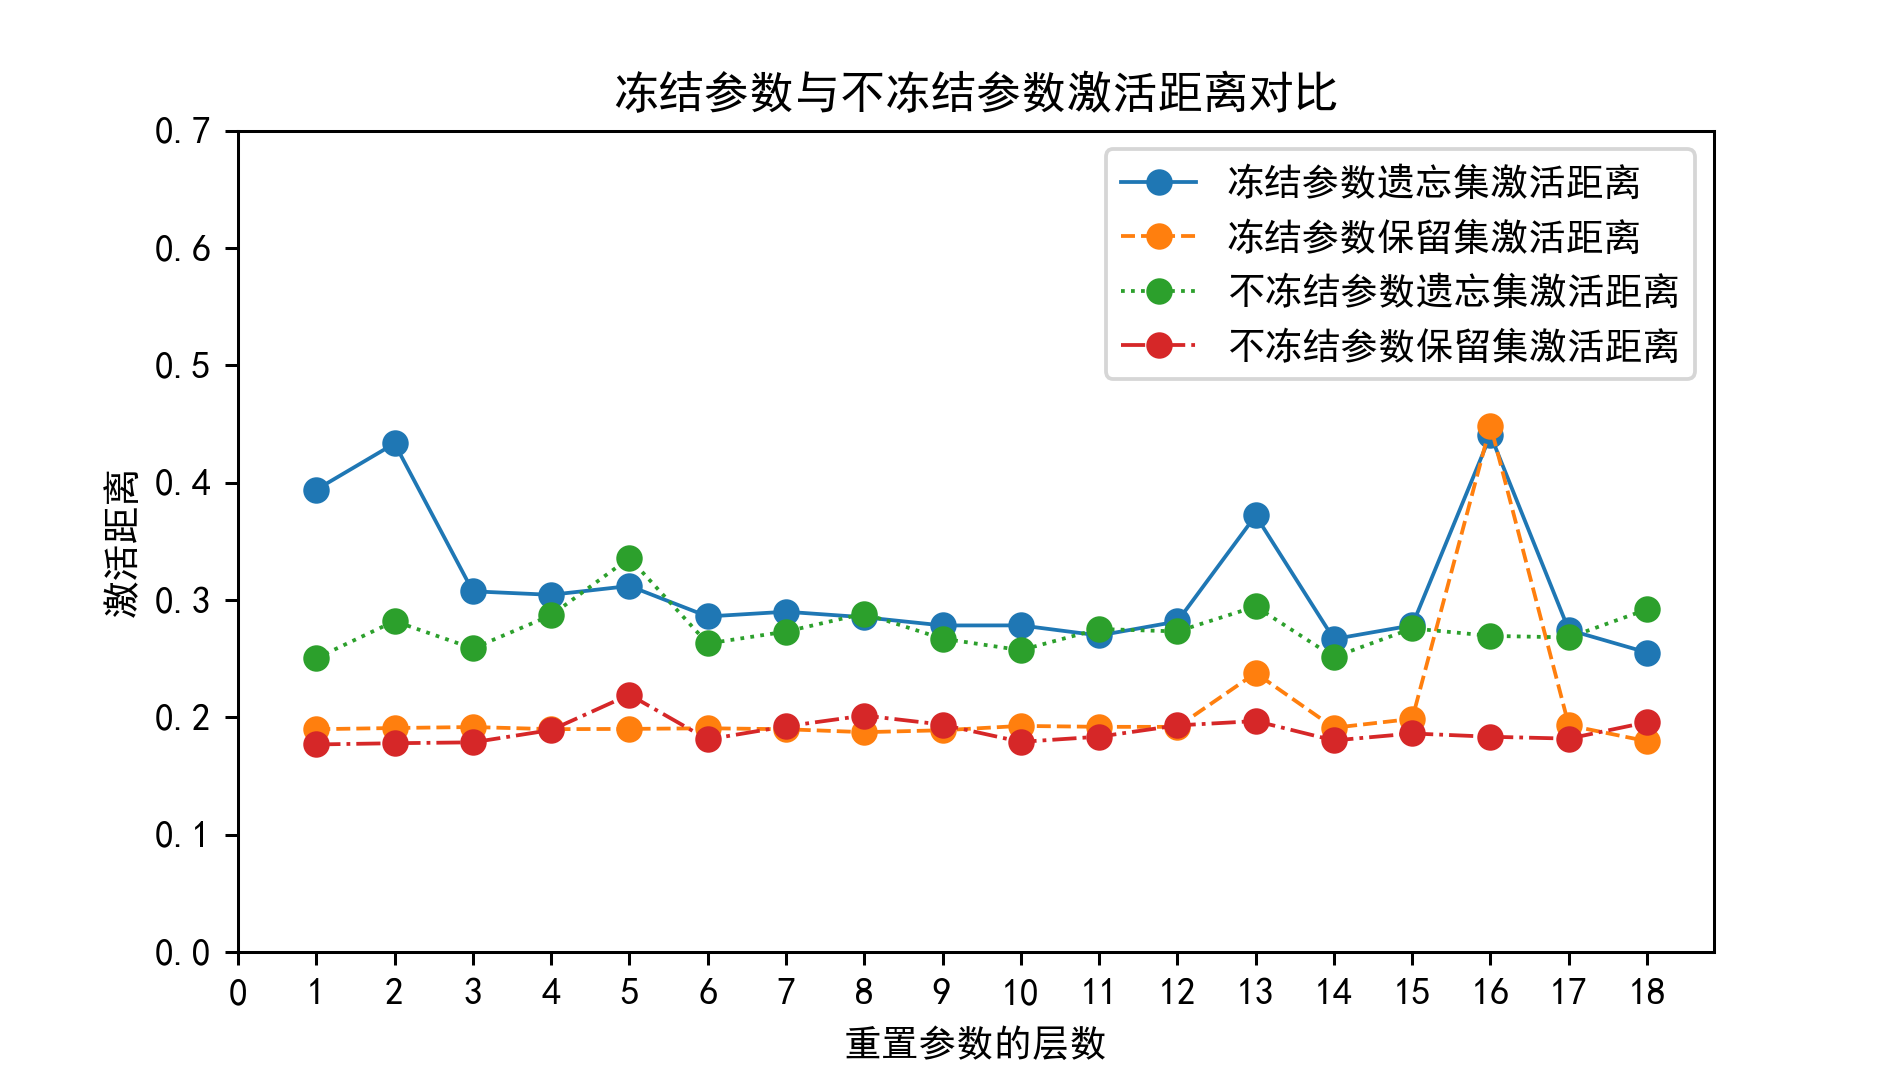
\includegraphics[width=0.9\linewidth]{chapter4_distance_2.png}
    \caption{冻结参数与没冻结参数激活距离对比}
    \label{fig:chapter4_distance_2}
\end{figure}
\subsection{反向冻结验证实验}
\begin{figure}
    \centering
    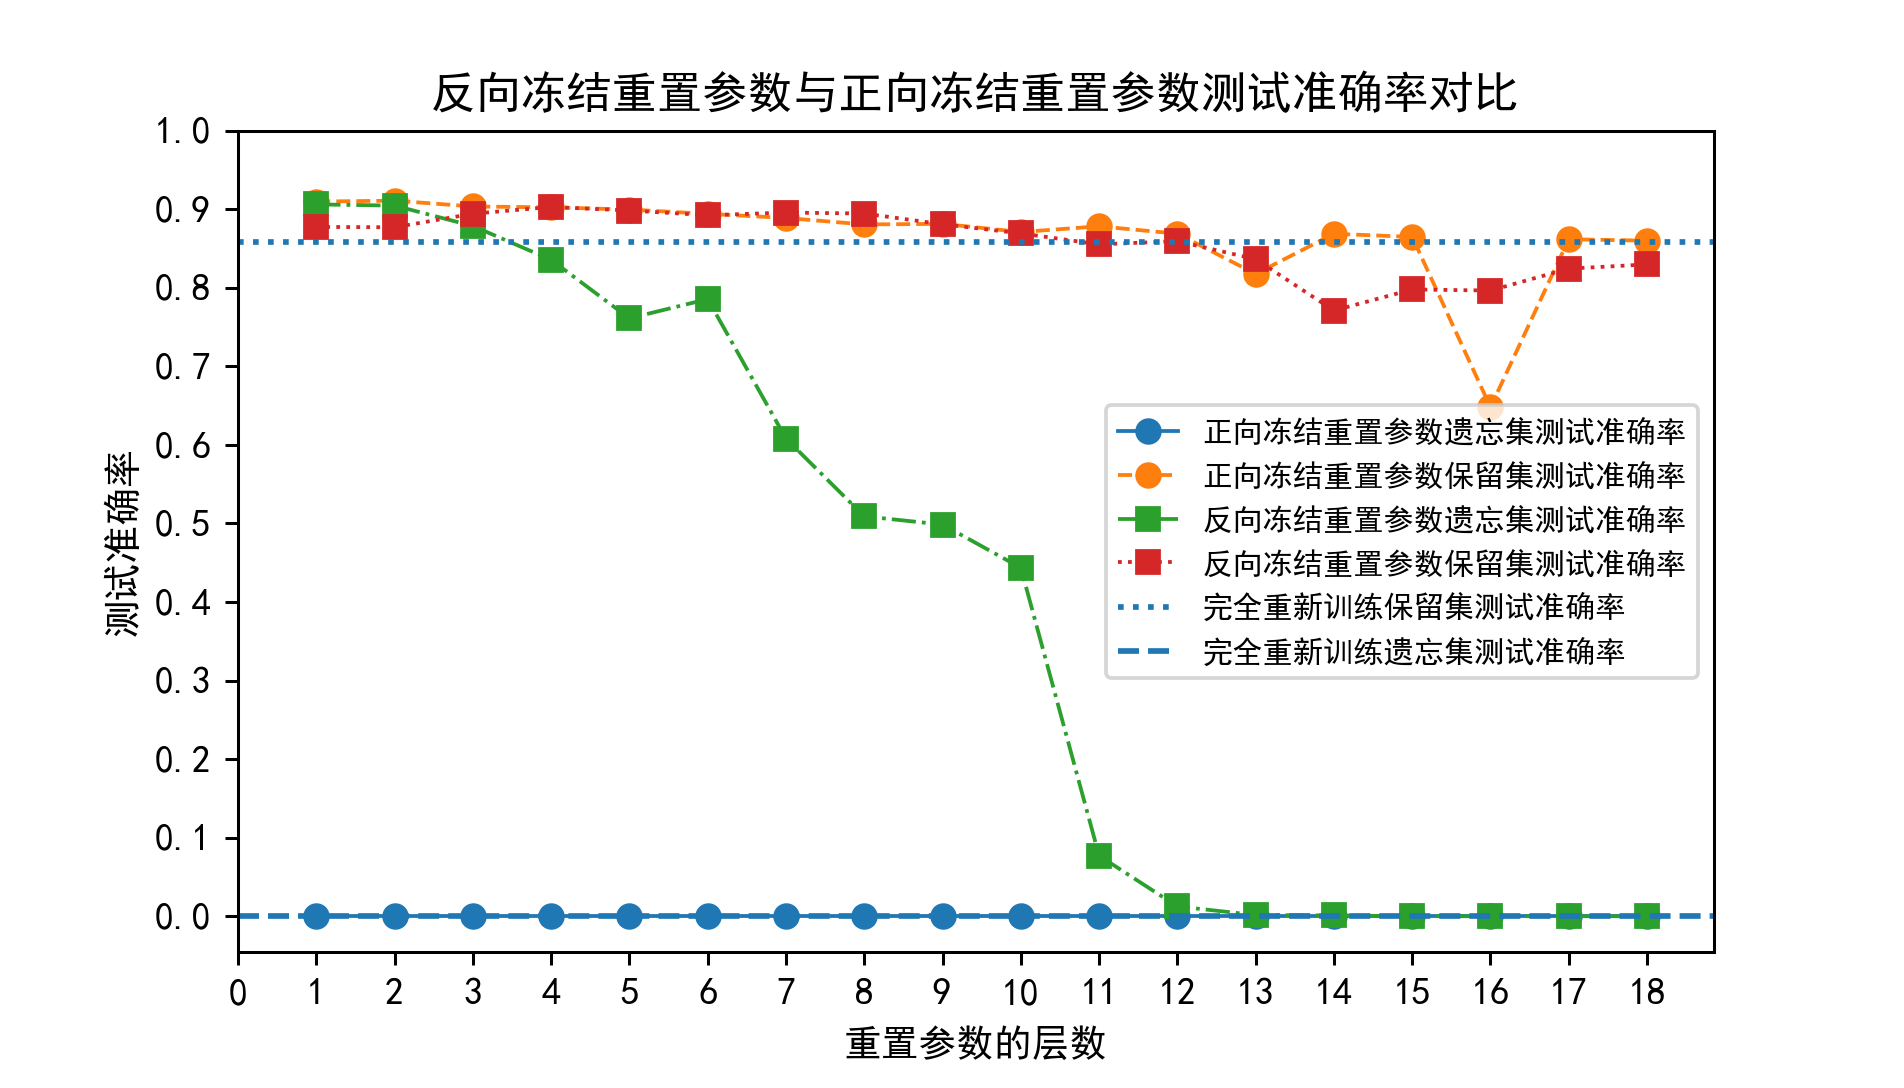
\includegraphics[width=0.9\linewidth]{chapter4_3.png}
    \caption{反向冻结重置参数与正向冻结重置参数测试准确率对比}
    \label{fig:chapter4_3}
\end{figure}
\begin{figure}
    \centering
    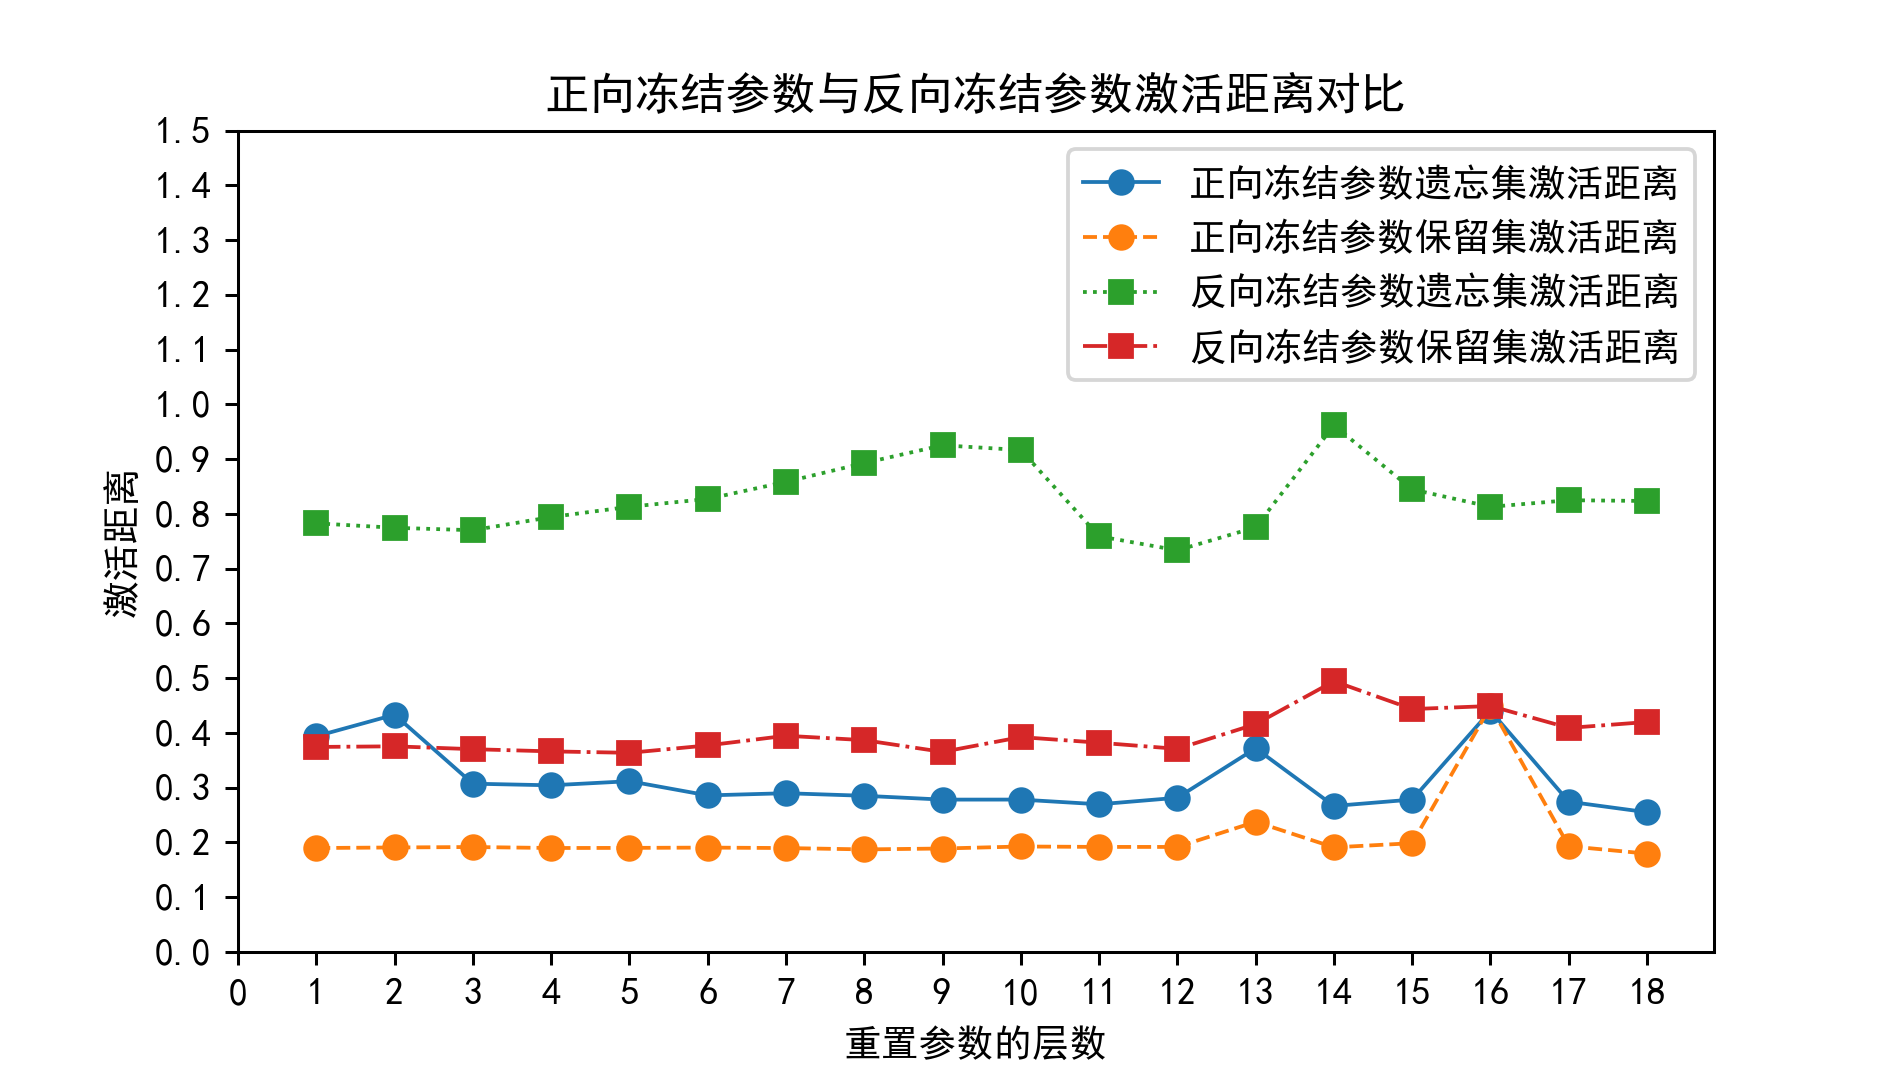
\includegraphics[width=0.9\linewidth]{chapter4_distance_3.png}
    \caption{正向冻结参数与反向冻结参数激活距离对比}
    \label{fig:chapter4_distance_3}
\end{figure}
\subsection{遗忘可持续性验证实验}
\begin{figure}
    \centering
    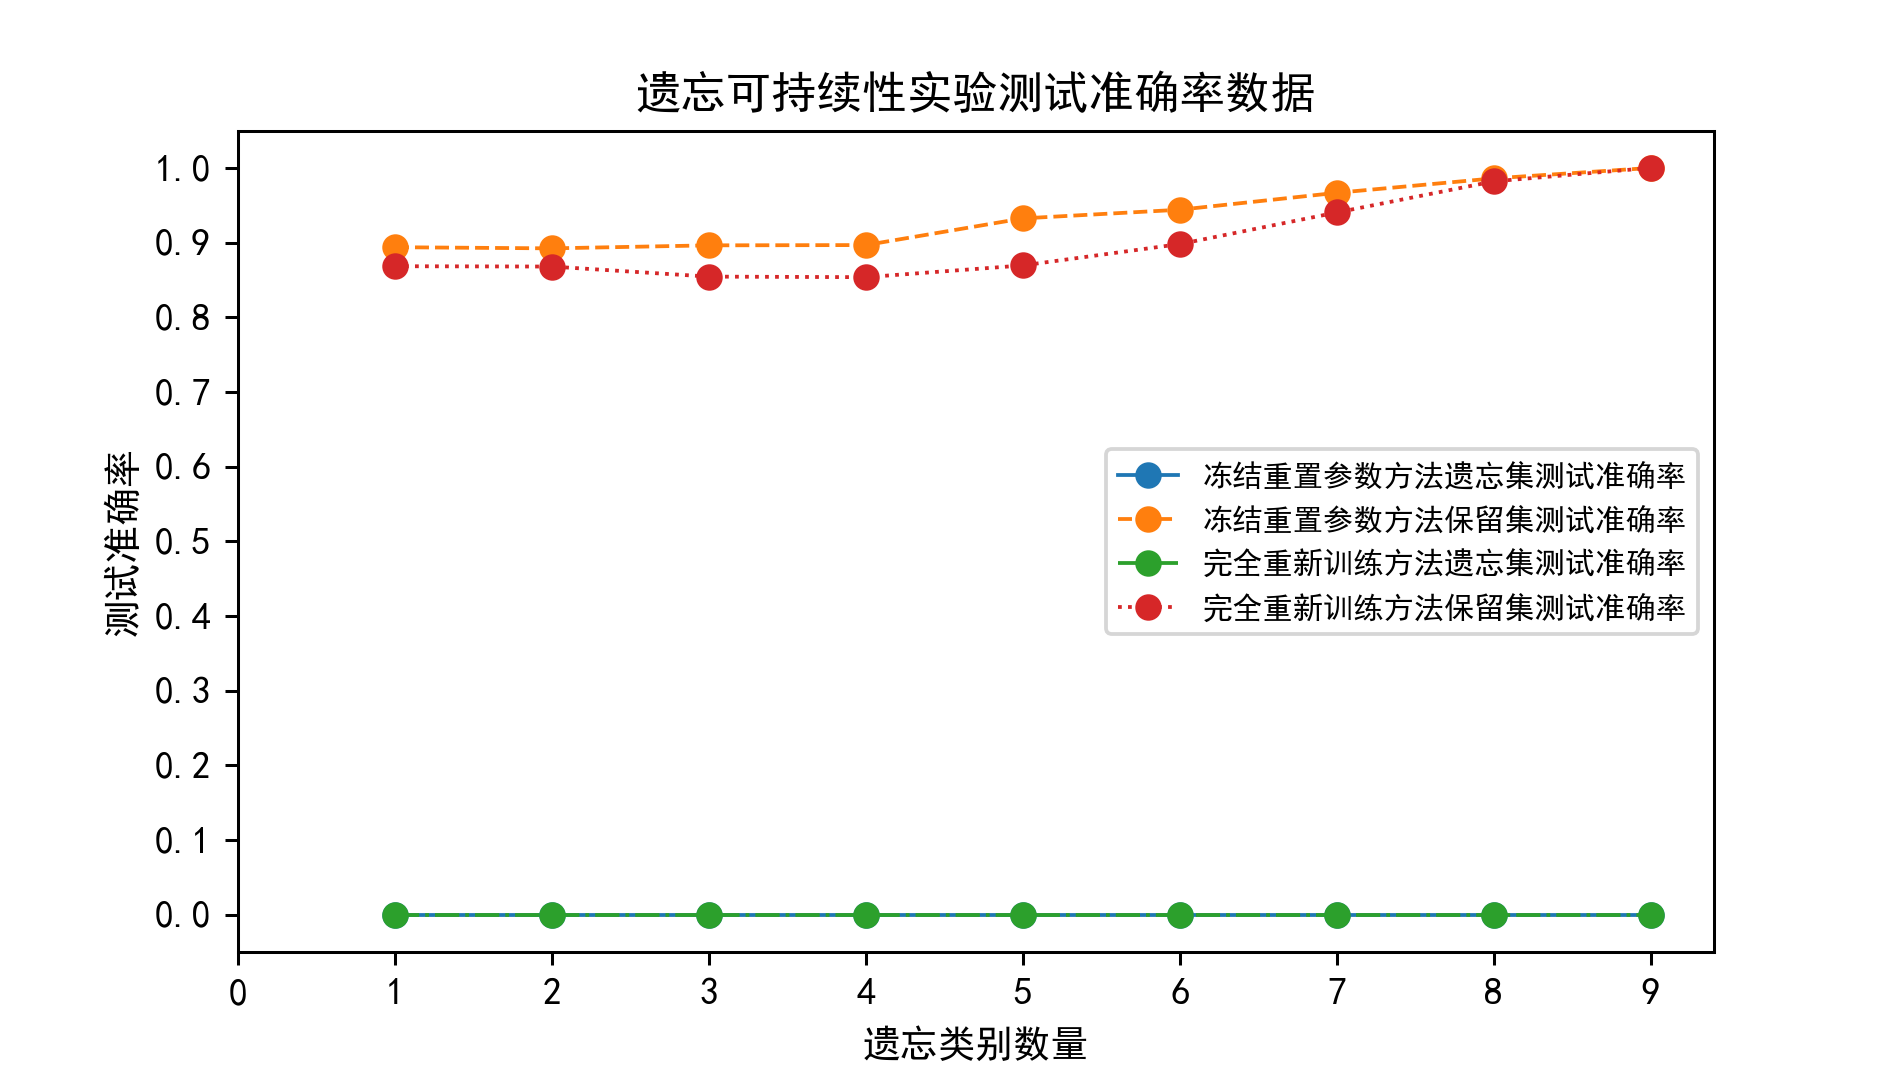
\includegraphics[width=0.9\linewidth]{chapter4_4.png}
    \caption{遗忘可持续性实验测试准确率数据}
    \label{fig:chapter4_4}
\end{figure}
\begin{figure}
    \centering
    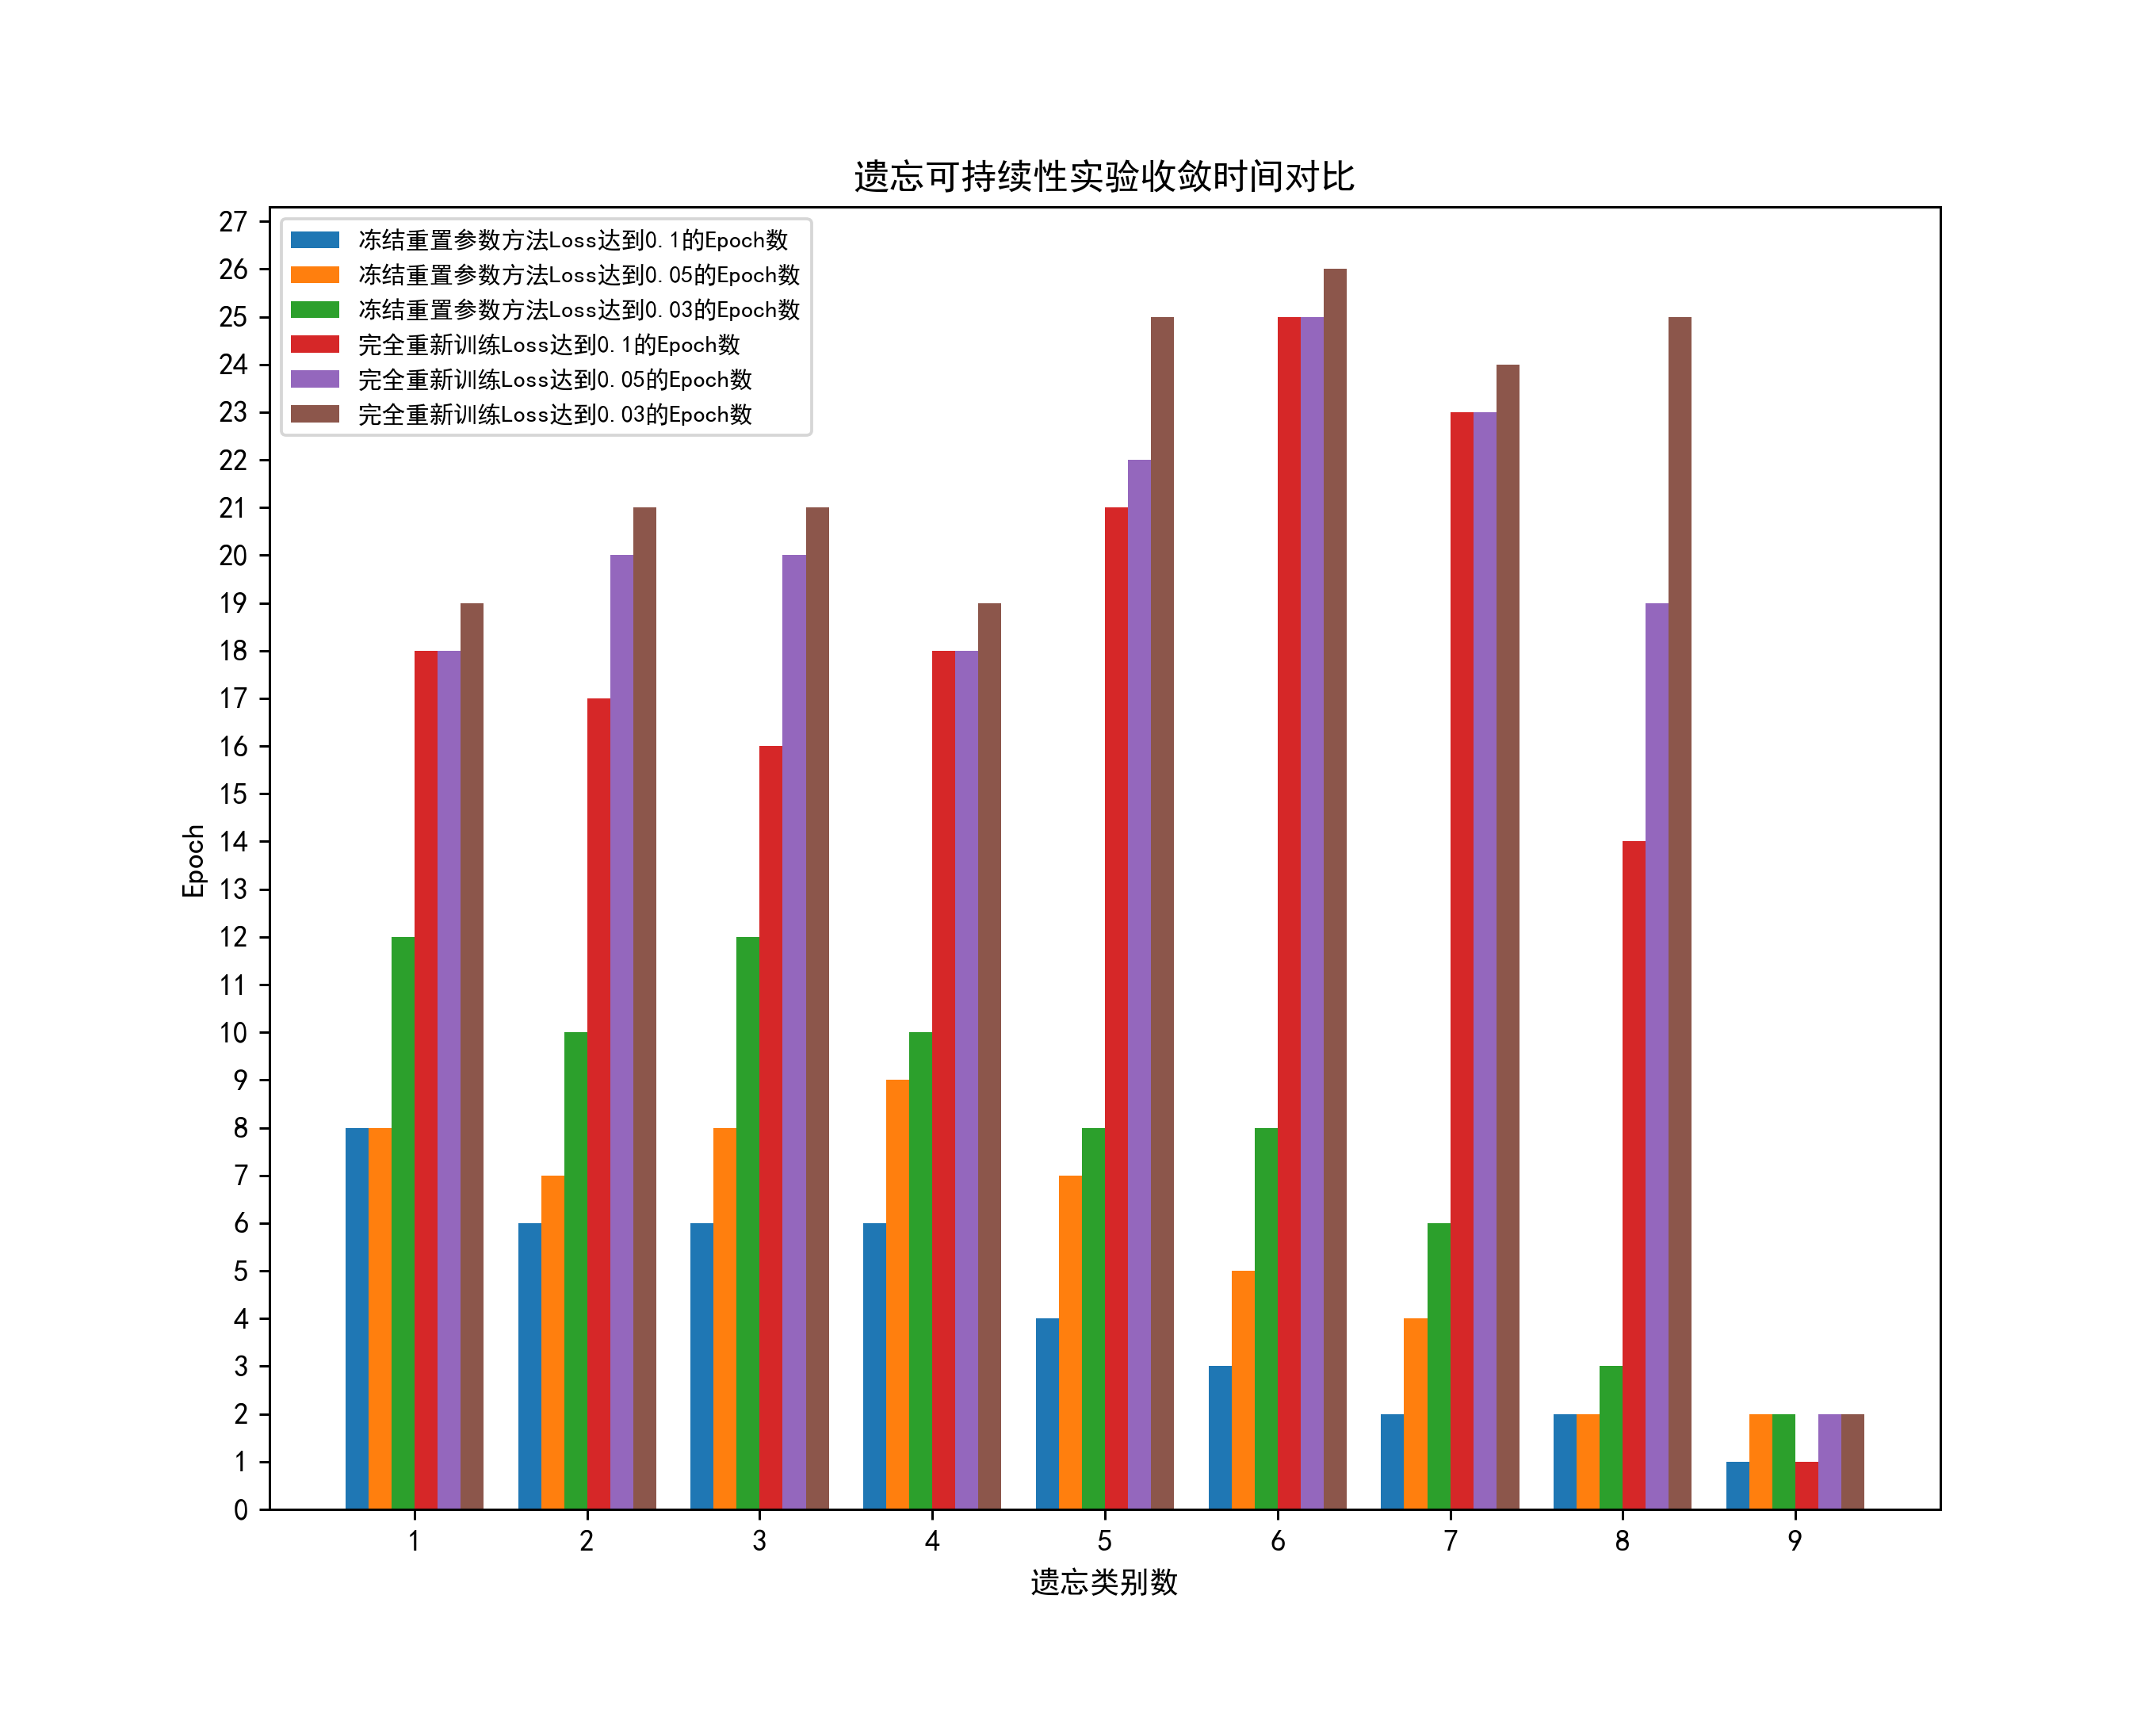
\includegraphics[width=1\linewidth]{chapter4_time_3.png}
    \caption{遗忘可持续性实验收敛时间对比}
    \label{fig:chapter4_time_3}
\end{figure}
\begin{figure}
    \centering
    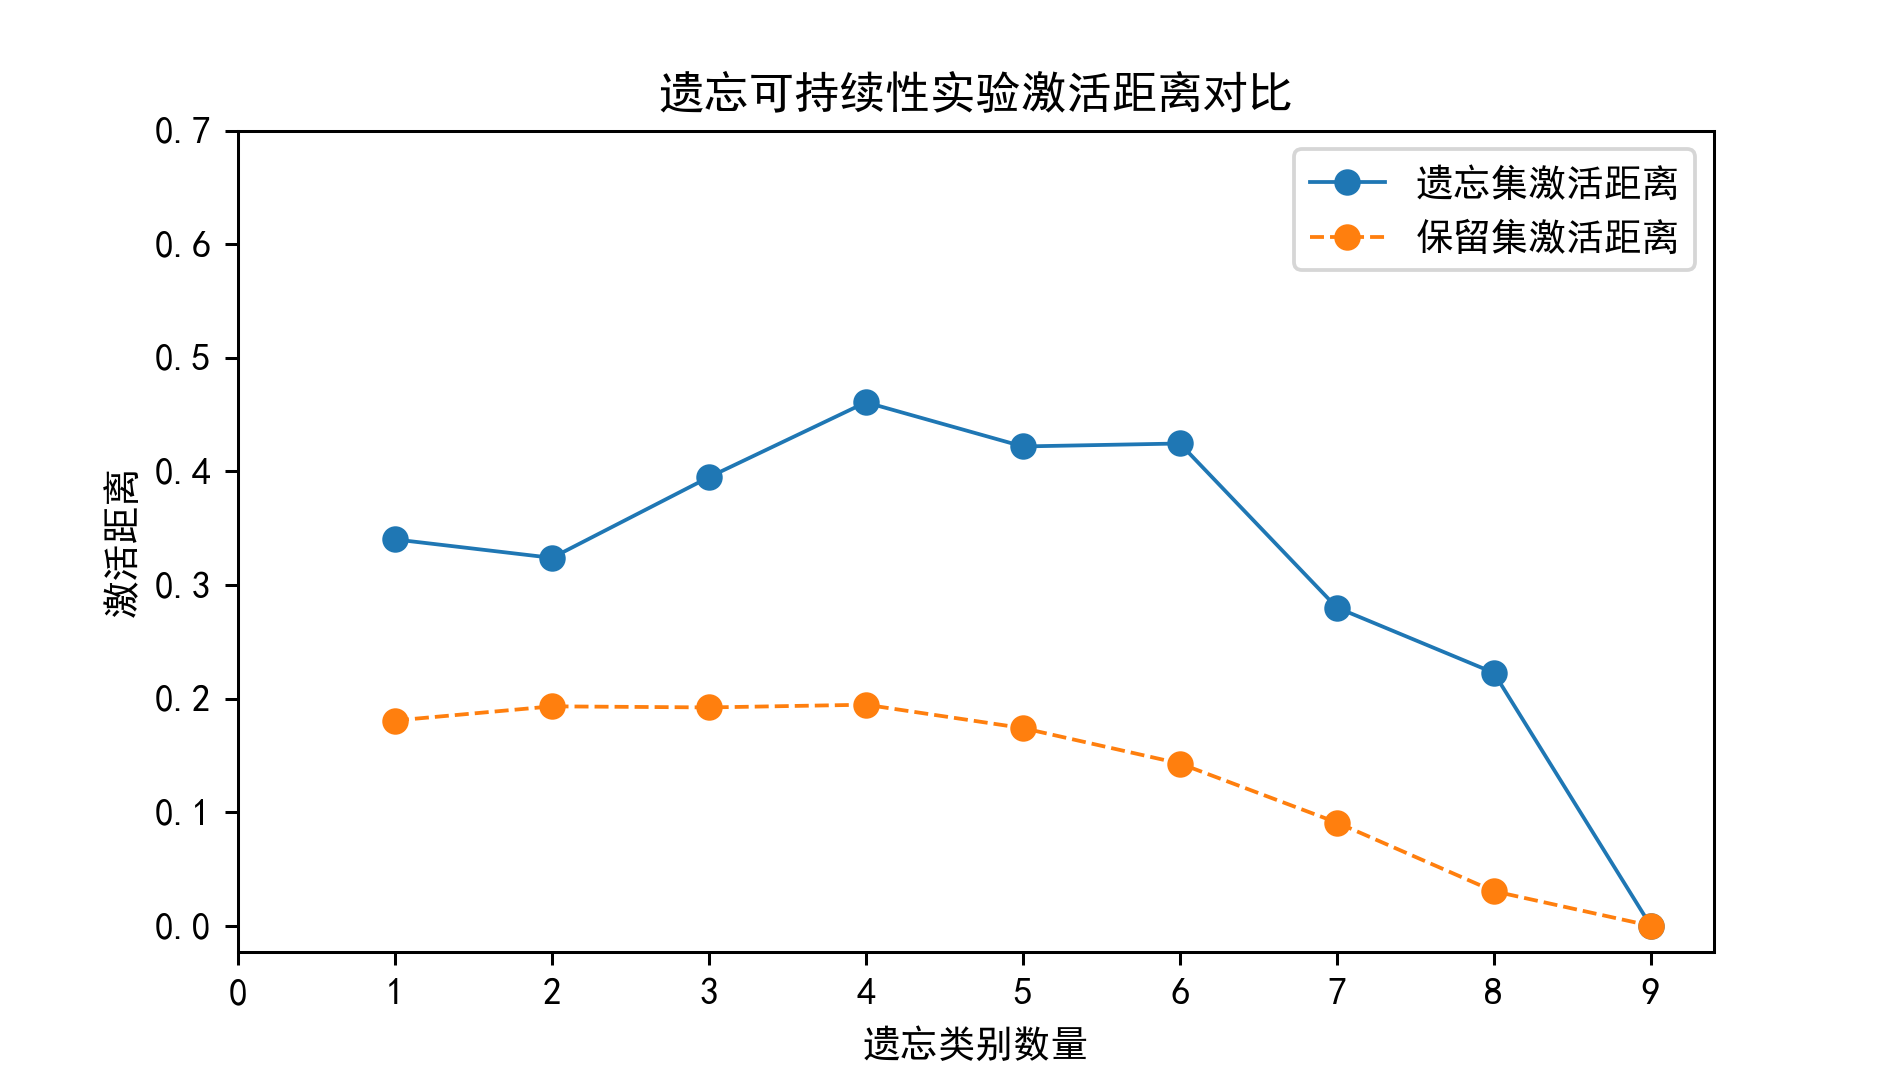
\includegraphics[width=0.9\linewidth]{chapter4_distance_4.png}
    \caption{遗忘可持续性实验激活距离对比}
    \label{fig:chapter4_distance_4}
\end{figure}
\section{本章小结}

